% SCARA course project report. Compile main.tex with pdfLaTeX on Overleaf,
% or run: tectonic main.tex
% Keep figures/ and results/ next to this file. No shell escape or BibTeX needed.
\documentclass[11pt,a4paper]{article}
\usepackage[T1]{fontenc}
\usepackage[utf8]{inputenc}
\usepackage{lmodern}
\usepackage[margin=25mm,headheight=14pt]{geometry}
\usepackage{amsmath,amssymb,bm}
\usepackage{graphicx,booktabs,tabularx,array}
\usepackage{tikz}
\usetikzlibrary{arrows.meta,calc}
\usepackage{caption,subcaption,float,placeins}
\usepackage{fancyhdr,microtype,enumitem}
\usepackage[hidelinks]{hyperref}
\usepackage{url}
\urlstyle{tt}
\graphicspath{{figures/}}
\hypersetup{pdftitle={SCARA Robot Manipulator: Modelling, Control and Motion Planning},
 pdfauthor={Ronit Ranjan, Pushkar Gudla, Harshvardhan Patidar, Adishesh Balaji}}
\pagestyle{fancy}
\fancyhf{}
\fancyhead[L]{\small SCARA Robot Manipulator}
\fancyhead[R]{\small AI4000: Robotics}
\fancyfoot[C]{\thepage}
\renewcommand{\headrulewidth}{0.4pt}
\setlength{\parindent}{0pt}
\setlength{\parskip}{5pt plus 1pt}
\setlength{\emergencystretch}{2em}
\raggedbottom
\makeatletter
\setlength{\@fptop}{0pt}
\setlength{\@fpsep}{14pt}
\makeatother
\setcounter{tocdepth}{2}
\setlist[itemize]{topsep=3pt,itemsep=2pt,leftmargin=*}
\setlist[enumerate]{topsep=3pt,itemsep=2pt,leftmargin=*}
\captionsetup{font=small,labelfont=bf,skip=6pt}
\captionsetup[subfigure]{font=small}
\renewcommand{\arraystretch}{1.15}
\newcolumntype{Y}{>{\raggedright\arraybackslash}X}
\newcommand{\R}{\mathbb{R}}
\newcommand{\dd}{\mathrm{d}}
% Primitive input keeps generated table rows expandable inside alignments.
\makeatletter\let\inputrows\@@input\makeatother
\newcommand{\figfull}[4][0.95]{%
 \begin{figure}[htbp]\centering
 \includegraphics[width=#1\linewidth]{#2}\caption{#3}\label{#4}\end{figure}}
\begin{document}
\hypersetup{pageanchor=false}
\begin{titlepage}
\centering
\vspace*{8mm}
{\large Indian Institute of Technology Hyderabad\par}
\vspace{5mm}
{\large AI4000: Robotics\par}
\vspace{16mm}
{\Huge\bfseries SCARA Robot Manipulator\par}
\vspace{5mm}
{\Large Modelling, kinematics, dynamics, control,\par
 pick-and-place and motion planning in MuJoCo\par}
\vspace{10mm}
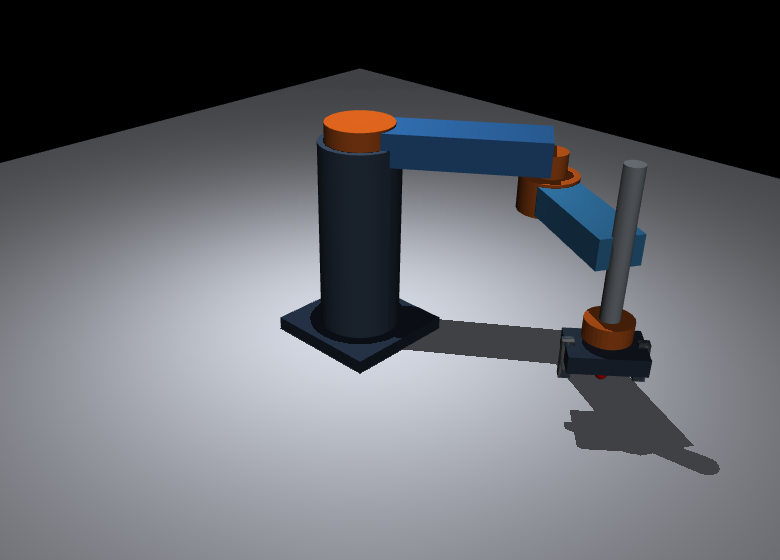
\includegraphics[width=.74\textwidth,height=62mm,keepaspectratio]{basemodel.png}
\vfill
\begin{tabular}{ll}
Ronit Ranjan & AI24BTECH11028\\
Pushkar Gudla & AI24BTECH11012\\
Harshvardhan Patidar & AI24BTECH11015\\
Adishesh Balaji & AI24BTECH11016
\end{tabular}
\vspace{12mm}

\begin{minipage}{.94\textwidth}
\hrule\vspace{6pt}
\textbf{Post-presentation addition.}
The RRT-Connect obstacle-avoidance path planner described in
Section~\ref{sec:rrt} was implemented \textbf{after feedback from the final
presentation}. It was not part of the implementation shown at that
presentation.
\vspace{6pt}\hrule
\end{minipage}
\vspace{8mm}
{\large Project report\par}
{\normalsize 27 November 2026\par}
\end{titlepage}

\pagenumbering{roman}
\hypersetup{pageanchor=true}
\section*{Abstract}
\addcontentsline{toc}{section}{Abstract}
This project develops a computer-only SCARA manipulator with an R--R--P--R
arm and an independently actuated parallel gripper. A parameterized geometry
model provides STL meshes, a URDF description and a MuJoCo XML model. The
mathematical model uses standard Denavit--Hartenberg parameters, closed-form
forward and inverse kinematics, a task Jacobian, inverse velocity kinematics
and an Euler--Lagrange dynamics model. Automated checks compare these
descriptions with MuJoCo's kinematic and dynamic quantities.

Synchronized time-scaling profiles and computed-torque control execute
motions within configured joint constraints. The task simulation picks up a
free 80 g block through frictional finger contact, carries it between two
stands and verifies grasp retention, clearance and final placement. An
eye-in-hand camera adds image-based visual servoing using four detected
corners and depth measurements before the grasp. Experiments include altered
depth estimates, camera mounting errors and an initially displaced object.

\textbf{After feedback from the final presentation, we implemented an
additional RRT-Connect path planner.} It searches for obstacle-avoiding
routes in joint space and accounts for the carried block during the
transfer. The report identifies this work separately from the original
timed waypoint trajectories. Thirteen seeded physical trials evaluate the
extension on the nominal obstacle and a shifted obstacle.

\textbf{Scope.} All results are from simulation. Dimensions, masses,
inertias, friction coefficients and motor limits are educational design
assumptions. Numerical agreement between mathematical models does not
establish the accuracy or safety of physical hardware.

\clearpage
\tableofcontents
\clearpage
\pagenumbering{arabic}

\section{Project objectives and implementation scope}
The objective is to connect the mathematical description of a SCARA robot
to a working manipulation task in MuJoCo~\cite{mujocodocs}. The mechanism follows
the R--R--P arm with a vertical rotary wrist used in the course
material~\cite{course}.
Its four task coordinates are horizontal position, vertical position and
tool yaw. The two gripper slides add grasp motion without changing the
four-dimensional arm task.

The project follows the checklist below:
\begin{enumerate}
 \item Define the robot geometry, joint limits, masses, frames, and sign conventions.
 \item Build the model and assign frames/DH parameters.
 \item Derive forward and inverse kinematics, including unreachable targets.
 \item Derive velocity kinematics (the Jacobian), and identify singularities.
 \item Derive forward and inverse dynamics from the robot's energies.
 \item Plan a timed path, then control the actuators to track it.
 \item Add a simulated task: objects, grasp/release, and collision constraints.
 \item Validate the equations and measure task results: tracking error, placement accuracy, effort, failures, and cycle time.
\end{enumerate}

There are two distinct planning stages in this report. The original project
provides timed trajectories through specified waypoints. The extension in
Section~\ref{sec:rrt} searches for the waypoints needed to avoid an obstacle.
The latter was added after final-presentation feedback and uses the same
physical robot, controller and grasp checks.

\subsection{Simulation workflow}
MuJoCo provides rigid-body dynamics, contact forces, camera rendering and
interactive visualization. The analytical kinematics and dynamics define
motion references and predicted behaviour. Trajectory generation sets
joint position, velocity and acceleration references; computed-torque
control converts them to motor efforts. Image feedback aligns the tool
before grasping, while collision and grasp checks monitor the task.

\section{Robot model and design parameters}\label{sec:model}
\subsection{Geometry and model generation}
The model uses boxes for the arm links, palm and fingers, and cylinders for
the pedestal, hubs and slide shaft. A parameterized construction defines
the mesh vertices and triangular faces and assembles the parent--child
link hierarchy in MuJoCo. Mesh geometry determines
appearance, while the body hierarchy, joint definitions, inertial elements
and collision geometries define simulation behaviour.

The model has six scalar joints: shoulder, elbow, vertical slide, wrist,
left finger and right finger. Direct-effort motors actuate these joints.
An additional free joint represents the independent payload in the task
scene. The payload receives forces through contact with the fingers and
stands.

The solid geometry was modelled parametrically in FreeCAD using box and
cylindrical primitives~\cite{freecad}. STL meshes provide the visual
geometry, while STEP supports solid-model exchange. The joint arrangement,
inertial properties and collision geometry are defined in MuJoCo.
The collision-clearance correction and all reported simulation results
were evaluated on the MuJoCo assembly.

\subsection{Dimensions and limits}
\begin{table}[htbp]\centering
\caption{Geometric design parameters. The mathematical model uses SI units.}\label{tab:geometry}
\begin{tabular}{@{}lll@{}}\toprule
Parameter & Value & Meaning\\\midrule
$h$ & 280 mm & World height of DH frame 0\\
$a_1$ & 240 mm & Shoulder-to-elbow axis distance\\
$a_2$ & 180 mm & Elbow-to-slide axis distance\\
$d_{3,0}$ & 80 mm & Slide reference offset at $q_3=0$\\
$q_3$ stroke & 0--110 mm & Additional downward travel\\
$d_4$ & 75 mm & Wrist reference to tool point\\
Forearm mesh offset & $-52$ mm & Vertical offset of the forearm solid\\
Gripper opening & 44--80 mm & Gap between the inner finger faces\\
\bottomrule\end{tabular}\end{table}

\begin{table}[htbp]\centering
\caption{Configured joint position, speed and motor-effort limits.}\label{tab:limits}
\begin{tabular}{@{}llll@{}}\toprule
Joint & Position range & Speed limit & Effort limit\\\midrule
Shoulder & $\pm150^\circ$ & 6 rad/s & 12 N m\\
Elbow & $\pm145^\circ$ & 8 rad/s & 8 N m\\
Vertical & 0--110 mm & 0.8 m/s & 80 N\\
Wrist & $\pm180^\circ$ & 12 rad/s & 2 N m\\
Each finger & 0--18 mm & 0.25 m/s & 8 N\\
\bottomrule\end{tabular}\end{table}

The ABB IRB 920T-6/0.45 serves as an industrial reference for the joint
travel limits. Its published shoulder and elbow working ranges are
$\pm150^\circ$ and $\pm145^\circ$, respectively, matching the ranges
chosen here~\cite{abb}. Link dimensions, slide stroke, wrist travel,
speeds and motor efforts remain project design choices.

The finite elbow range excludes the fully folded $180^\circ$ configuration.
It does not exclude the straight-arm singularity at $q_2=0$, so numerical
motion methods still need singularity handling. Finite rotary ranges are
intervals: the planner does not wrap an angle through a mechanical stop.
The speed limits are checked by trajectory generation and execution
monitoring; they are not automatically enforced by a direct-effort motor.

With $a_1+a_2=420$ mm, the arm has a 420 mm geometric outer reach. The elbow
limit raises the minimum reachable radius from the unconstrained
$|a_1-a_2|=60$ mm to approximately 138.7 mm. The shoulder limit further
restricts angular coverage. The vertical tool range is 15--125 mm above the
floor. These are design consequences, rather than evidence that the model
has been optimized for a particular industrial installation.

\subsection{Mass and inertia assumptions}
\begin{table}[htbp]\centering
\caption{Assigned moving masses. The base and payload are excluded.}\label{tab:masses}
\begin{tabular}{@{}lr@{}}\toprule
Component & Mass (kg)\\\midrule
Upper arm & 1.10\\
Forearm & 0.75\\
Vertical carriage & 0.30\\
Wrist and palm & 0.22\\
Each finger & 0.04\\\midrule
Total moving robot mass & 2.45\\
\bottomrule\end{tabular}\end{table}

Masses and moments of inertia are specified explicitly. They are not
measurements and were not computed from an assigned CAD material density.
The slide carries the carriage, wrist, palm and both fingers, giving an
unloaded vertically moving mass of 0.60 kg. The analytical arm dynamics hold
the finger opening fixed and combine the wrist, palm and fingers into one
equivalent body. The physical grasp simulation retains the finger joints
and the free payload.

\subsection{Arm self-collision correction}
An earlier geometry placed the upper arm and forearm in the same plane.
At large elbow angles the solids intersected. Default contact filtering
between adjacent bodies did not reveal this interface, so relying only on
the active contact list was insufficient.

The corrected forearm solid and its centre of mass are 52 mm below the
original plane, joined through an elbow pin. The upper arm is 44 mm thick
and the forearm is 38 mm thick. Their half-thicknesses and the selected
clearance give
\begin{equation}
 \Delta z=\frac{44}{2}+11+\frac{38}{2}=52\ \mathrm{mm}.
\end{equation}
An explicit upper-arm/forearm collision pair supplements independent signed
distance checks. The joint-axis reference origins remain unchanged, so the
DH offsets and tool-height equation remain the same. The 52 mm solid offset
must not be subtracted again from the DH tool position.

\begin{figure}[htbp]\centering
\begin{subfigure}{.45\linewidth}\centering
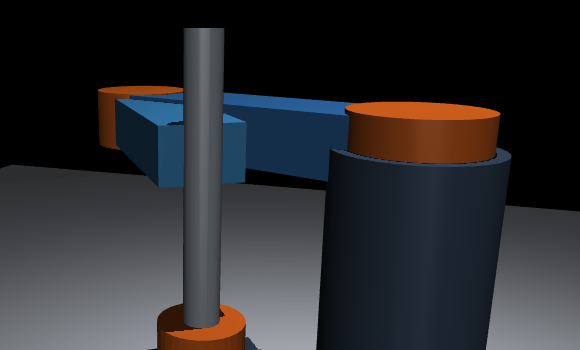
\includegraphics[width=\linewidth]{elbow_before.png}
\caption{Earlier coplanar solids at a large elbow angle.}
\end{subfigure}\hfill
\begin{subfigure}{.43\linewidth}\centering
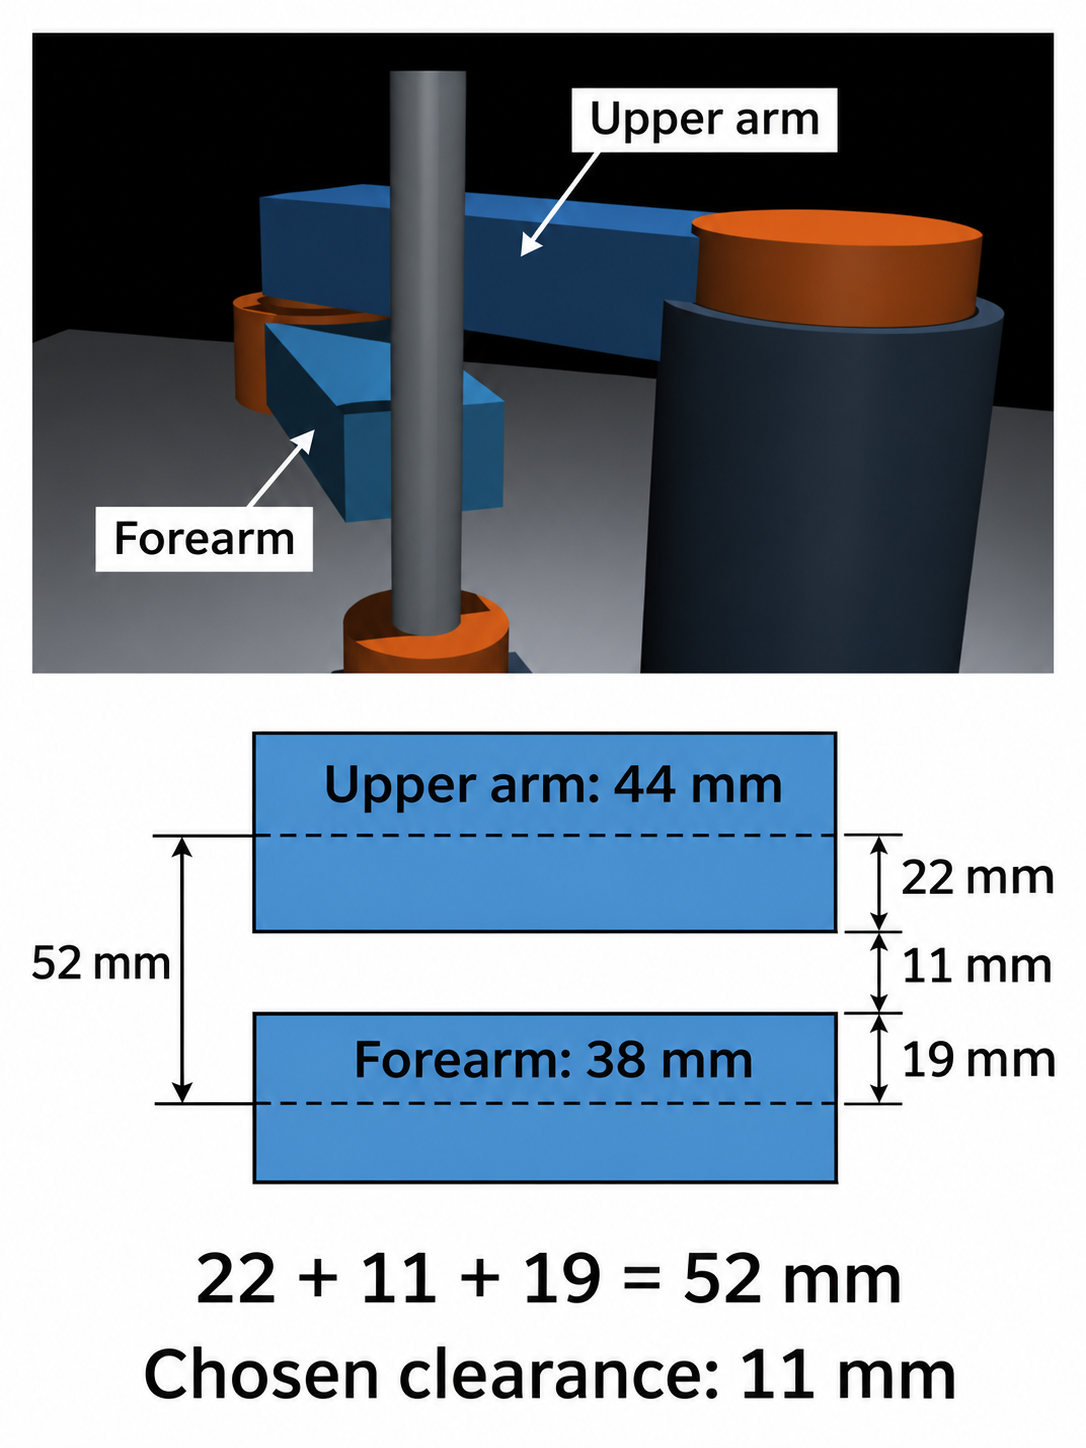
\includegraphics[width=\linewidth,height=78mm,keepaspectratio]{forearm_offset_52mm_vertical.png}
\caption{Corrected arrangement and the 52 mm separation.}
\end{subfigure}
\caption{The physical link offset resolves the arm-interface collision while preserving the joint reference frames. The dimension sketch is schematic.}\label{fig:offset}
\end{figure}
\FloatBarrier

\section{Frames and Denavit--Hartenberg description}\label{sec:dh}
\subsection{Frame assignment}
The assignment follows the class SCARA arrangement. Axes $z_0,z_1$ point
upward. A $180^\circ$ twist in the second DH transform makes $z_2,z_3,z_4$
point downward. Thus increasing $q_3$ lowers the tool, and positive wrist
rotation is about a downward axis.

The frame drawing uses body and tool positions obtained by running
MuJoCo forward kinematics at a selected pose. These positions are combined
with the chosen DH axis orientations and projected into a two-dimensional
diagram.
MuJoCo supplies the body poses; the DH convention remains an explicit
modelling choice.

\begin{figure}[htbp]\centering
\begin{subfigure}{.40\linewidth}\centering
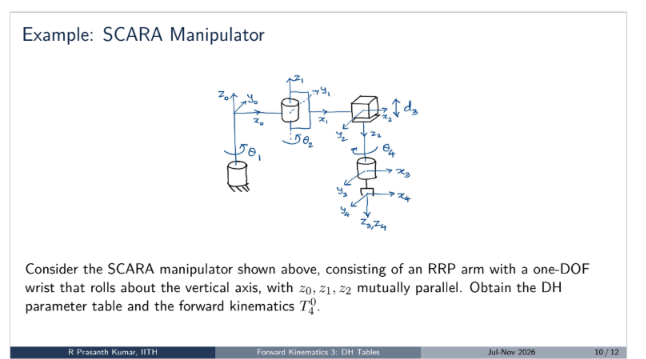
\includegraphics[width=\linewidth]{lecture_scara_frames.png}
\caption{Course reference arrangement.}
\end{subfigure}\hfill
\begin{subfigure}{.57\linewidth}\centering
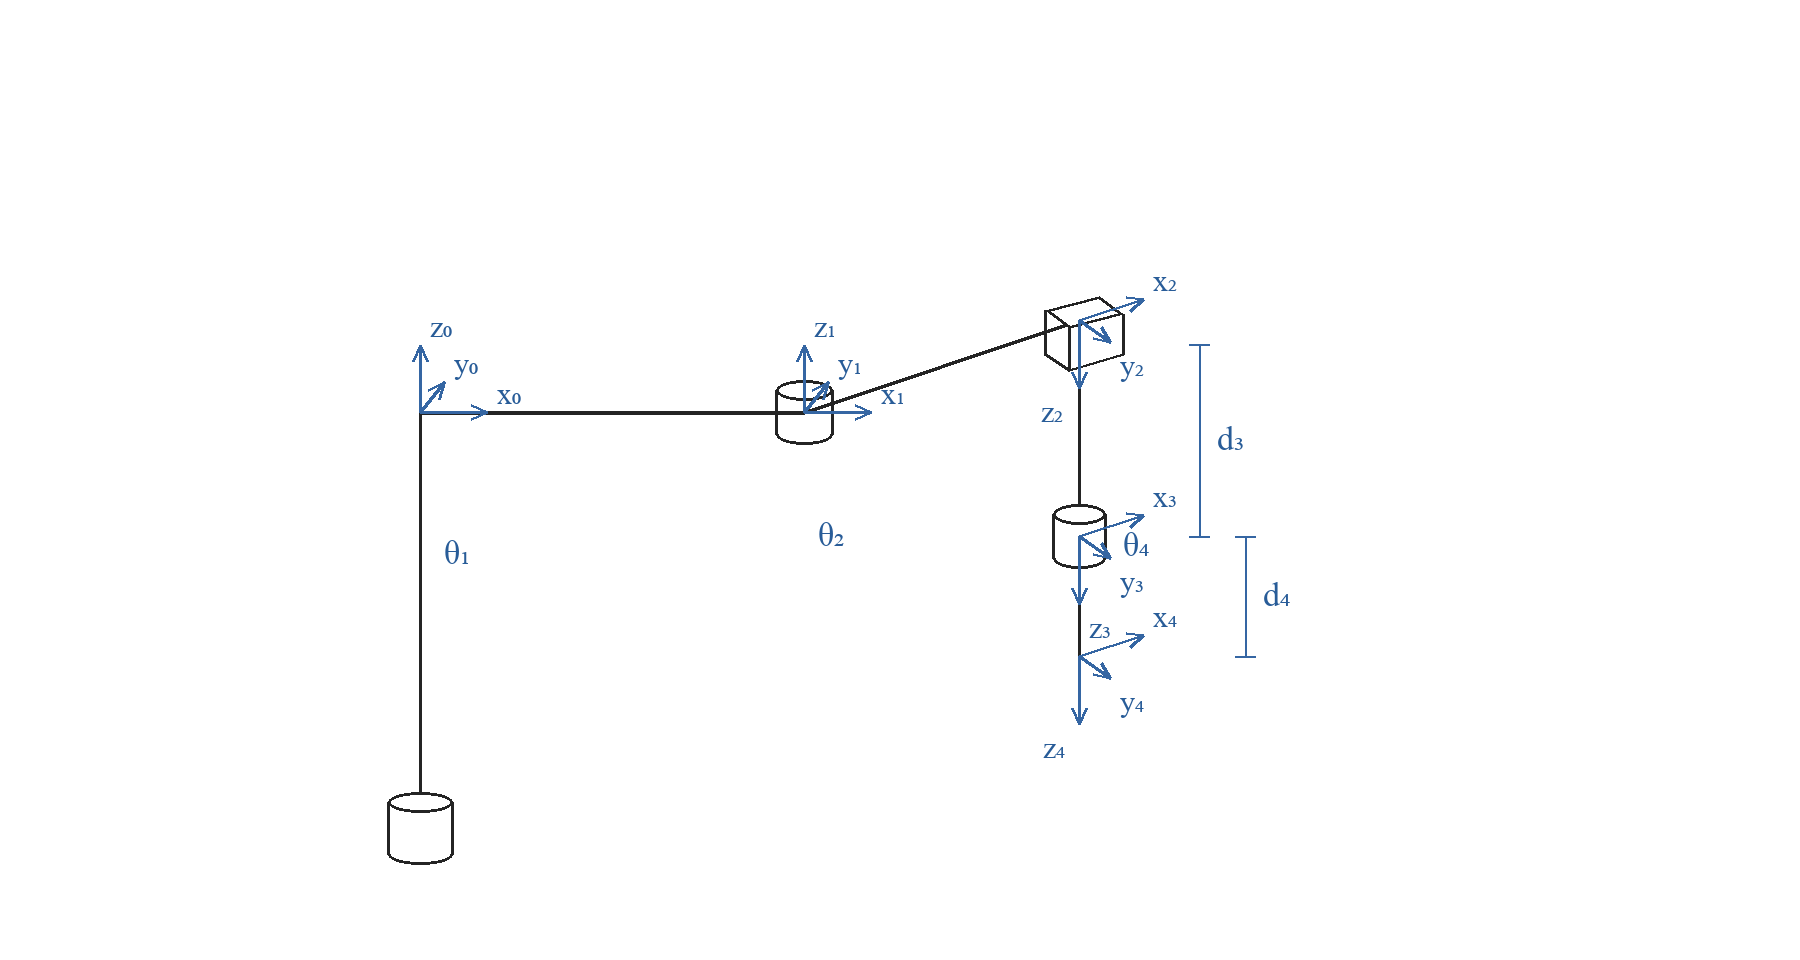
\includegraphics[width=\linewidth]{frame_assignment.png}
\caption{Assigned frames for the project model.}
\end{subfigure}
\caption{SCARA frame assignment. The course figure establishes the topology and convention; dimensions are project design values.}\label{fig:frames}
\end{figure}

\subsection{Standard DH table}
Let $q=[q_1,q_2,q_3,q_4]^T$, where $q_1,q_2,q_4$ are rotary coordinates and
$q_3$ is the simulator slide displacement. The slide's DH distance is
\begin{equation}
 d_3^*=d_{3,0}+q_3=0.080+q_3,\qquad 0\leq q_3\leq0.110\ \mathrm{m}.
\end{equation}
The reference offset $d_{3,0}$ is a geometric distance between frame origins.
It is not an 80 mm empty collision clearance.

\begin{table}[htbp]\centering
\caption{Standard DH parameters. Joint variables are $q_1,q_2,q_3,q_4$.}\label{tab:dh}
\begin{tabular}{@{}ccccc@{}}\toprule
$i$ & $a_i$ & $\alpha_i$ & $d_i$ & $\theta_i$\\\midrule
1 & $a_1$ & $0$ & $0$ & $q_1$\\
2 & $a_2$ & $\pi$ & $0$ & $q_2$\\
3 & $0$ & $0$ & $0.080+q_3$ & $0$\\
4 & $0$ & $0$ & $d_4$ & $q_4$\\
\bottomrule\end{tabular}\end{table}

The transform convention and world offset are
\begin{equation}
 A_i=R_z(\theta_i)T_z(d_i)T_x(a_i)R_x(\alpha_i),\qquad
 {}^WT_4=T_z(h)A_1A_2A_3A_4.
\end{equation}
The world-to-frame-0 translation is separate from the four DH rows because
frame 0 lies at shoulder height, rather than on the floor.

\subsection{Consistency with the simulator}
For the same joint values, the assembled robot's tool position is
obtained from MuJoCo forward kinematics. This model-derived world
position is compared with the position calculated from the DH transforms. The
acceptance threshold is $2\times10^{-7}$ m, or $0.2\,\mu$m. This is a
numerical consistency threshold, not a physical positioning-accuracy claim.

The DH tool axes include the downward-axis convention. The MuJoCo
construction tool axes differ by a fixed $R_x(\pi)$ rotation. A full pose
comparison must include that convention change. The separate kinematic
checks also form the homogeneous DH product explicitly.
\FloatBarrier

\section{Position and velocity kinematics}\label{sec:kinematics}
\subsection{Forward kinematics}
Using $c_1=\cos q_1$, $s_1=\sin q_1$ and
$c_{12}=\cos(q_1+q_2)$, $s_{12}=\sin(q_1+q_2)$, the task pose is
\begin{align}
 x&=a_1c_1+a_2c_{12},& y&=a_1s_1+a_2s_{12},\\
 z&=h-d_3^*-d_4,& \phi&=q_1+q_2-q_4.
\end{align}
The homogeneous transform in the DH orientation convention is
\begin{equation}
 {}^WT_4=\begin{bmatrix}
 \cos\phi&\sin\phi&0&x\\
 \sin\phi&-\cos\phi&0&y\\
 0&0&-1&z\\0&0&0&1
 \end{bmatrix}.
\end{equation}
At zero slide displacement the tool height is $280-80-75=125$ mm. At full
extension it is $280-190-75=15$ mm. The fingertips extend 5 mm below the tool
reference, leaving 10 mm above the floor at this limiting unloaded pose.

\subsection{Inverse kinematics and workspace}
For a desired tool pose $(x,y,z,\phi)$, the two rotary arm joints are first
found from the horizontal projection. Let $O$ be the shoulder, $E$ the elbow
and $P$ the tool-axis projection, so that $OE=a_1$, $EP=a_2$ and
$OP=r=\sqrt{x^2+y^2}$. Figure~\ref{fig:iktriangles} shows the arm triangle
and its components in axes aligned with the first link.

\begin{figure}[H]\centering
\begin{subfigure}[t]{.49\linewidth}\centering
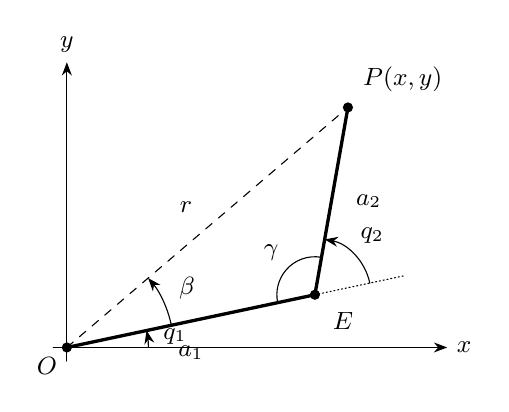
\begin{tikzpicture}[scale=1.15,>=Stealth,line cap=round,line join=round,
                    every node/.style={font=\small}]
 \coordinate (O) at (0,0);
 \coordinate (E) at ({2.8*cos(12)},{2.8*sin(12)});
 \coordinate (P) at ({2.8*cos(12)+2.1*cos(80)},
                     {2.8*sin(12)+2.1*sin(80)});
 \draw[->,thin] (-.15,0)--(4.2,0) node[right] {$x$};
 \draw[->,thin] (0,-.15)--(0,3.15) node[above] {$y$};
 \draw[very thick] (O)--node[midway,below=5pt] {$a_1$}(E)
                       --node[midway,right=5pt] {$a_2$}(P);
 \draw[dashed] (O)--node[midway,above left=2pt] {$r$}(P);
 \draw[densely dotted] (E)--++({1.0*cos(12)},{1.0*sin(12)});
 \draw[->] (.9,0) arc[start angle=0,end angle=12,radius=.9];
 \node at ({1.20*cos(6)},{1.20*sin(6)}) {$q_1$};
 \draw[->] ({1.18*cos(12)},{1.18*sin(12)})
       arc[start angle=12,end angle=40.5,radius=1.18];
 \node at ({1.48*cos(26.25)},{1.48*sin(26.25)}) {$\beta$};
 \draw[->] ($(E)+({.62*cos(12)},{.62*sin(12)})$)
       arc[start angle=12,end angle=80,radius=.62];
 \node at ($(E)+({.91*cos(46)},{.91*sin(46)})$) {$q_2$};
 \draw ($(E)+({.42*cos(80)},{.42*sin(80)})$)
       arc[start angle=80,end angle=192,radius=.42];
 \node at ($(E)+({.67*cos(136)},{.67*sin(136)})$) {$\gamma$};
 \fill (O) circle (1.6pt) node[below left] {$O$};
 \fill (E) circle (1.6pt) node[below right=3pt] {$E$};
 \fill (P) circle (1.6pt) node[above right=2pt] {$P(x,y)$};
\end{tikzpicture}
\caption{Horizontal arm triangle, shown for $q_2>0$.}
\end{subfigure}\hfill
\begin{subfigure}[t]{.49\linewidth}\centering
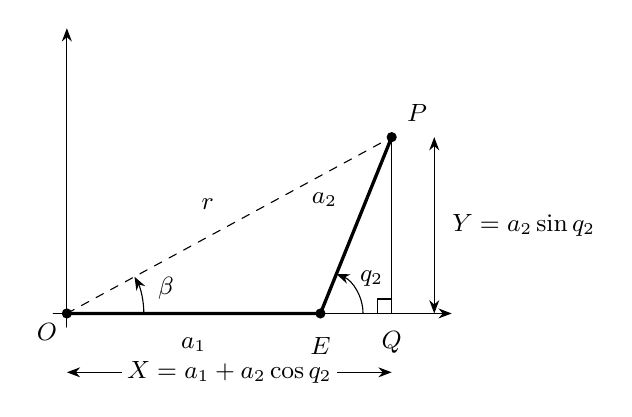
\begin{tikzpicture}[scale=1.15,>=Stealth,line cap=round,line join=round,
                    every node/.style={font=\small}]
 \coordinate (O) at (0,0);
 \coordinate (E) at (2.8,0);
 \coordinate (P) at ({2.8+2.1*cos(68)},{2.1*sin(68)});
 \coordinate (Q) at ({2.8+2.1*cos(68)},0);
 \draw[->,thin] (-.15,0)--(4.25,0);
 \draw[->,thin] (0,-.15)--(0,3.15);
 \draw[very thick] (O)--node[midway,below=5pt] {$a_1$}(E)
                       --node[midway,above left=3pt] {$a_2$}(P);
 \draw[dashed] (O)--node[midway,above left=2pt] {$r$}(P);
 \draw[thin] (P)--(Q);
 \draw ($(Q)+(-.16,0)$)--++(0,.16)--++(.16,0);
 \draw[->] (.85,0) arc[start angle=0,end angle=28.5,radius=.85];
 \node at ({1.13*cos(14.25)},{1.13*sin(14.25)}) {$\beta$};
 \draw[->] ($(E)+(.47,0)$) arc[start angle=0,end angle=68,radius=.47];
 \node at ($(E)+({.68*cos(34)},{.68*sin(34)})$) {$q_2$};
 \draw[<->,thin] (0,-.65)--node[midway,fill=white,inner sep=2pt]
          {$X=a_1+a_2\cos q_2$} ($(Q)+(0,-.65)$);
 \draw[<->,thin] ($(Q)+(.47,0)$)--node[midway,right=3pt]
          {$Y=a_2\sin q_2$} ($(P)+(.47,0)$);
 \fill (O) circle (1.6pt) node[below left] {$O$};
 \fill (E) circle (1.6pt) node[below=5pt] {$E$};
 \fill (P) circle (1.6pt) node[above right=2pt] {$P$};
 \node[below=3pt] at (Q) {$Q$};
\end{tikzpicture}
\caption{Right triangle after rotating the axes by $q_1$.}
\end{subfigure}
\caption{Geometry for inverse kinematics. The base-to-target bearing is
$\theta=\operatorname{atan2}(y,x)=q_1+\beta$. The internal elbow angle is
$\gamma=\pi-|q_2|$. Both diagrams are horizontal projections; the physical
52 mm offset between the arm solids does not change these triangles.}
\label{fig:iktriangles}
\end{figure}

\paragraph{Elbow angle from the cosine rule.}
In triangle $OEP$, the internal angle $\gamma$ is supplementary to the
magnitude of the signed joint angle $q_2$. Applying the cosine rule gives
\begin{align}
 r^2&=a_1^2+a_2^2-2a_1a_2\cos\gamma,\\
 \cos\gamma&=\cos(\pi-|q_2|)=-\cos q_2,\\
 r^2&=a_1^2+a_2^2+2a_1a_2\cos q_2.
\end{align}
Therefore,
\begin{equation}
 c_2\equiv\cos q_2=\frac{x^2+y^2-a_1^2-a_2^2}{2a_1a_2},\qquad
 \boxed{q_2=\pm\arccos c_2}.
\end{equation}
The two signs give the two elbow configurations reaching the same
horizontal point. A real solution requires $|c_2|\leq1$, equivalently
$|a_1-a_2|\leq r\leq a_1+a_2$. The solutions coincide when the triangle
becomes collinear.

\paragraph{Shoulder angle from the right triangle.}
In the first-link-aligned axes of Figure~\ref{fig:iktriangles}(b), the
target has signed components
\begin{equation}
 X=a_1+a_2\cos q_2,\qquad Y=a_2\sin q_2.
\end{equation}
The target bearing in these axes is $\beta=\operatorname{atan2}(Y,X)$.
The first link is rotated by $q_1$ relative to the world $x$ axis, so
\begin{equation}
 \theta=q_1+\beta,\qquad \theta=\operatorname{atan2}(y,x).
\end{equation}
Subtracting the two bearings gives
\begin{equation}
 \boxed{q_1=\operatorname{atan2}(y,x)
 -\operatorname{atan2}(a_2\sin q_2,a_1+a_2\cos q_2)}.
\end{equation}
This expression is evaluated for each sign of $q_2$. The signed sine and
the two-argument arctangent preserve the quadrant, including the negative
elbow configuration for which $Y$ and $\beta$ are negative.

\paragraph{Slide displacement and wrist angle.}
The vertical coordinate and tool yaw decouple from the arm triangle.
Substituting $d_3^*=d_{3,0}+q_3$ into the height equation gives
\begin{equation}
 z=h-(d_{3,0}+q_3)-d_4
 \quad\Longrightarrow\quad
 \boxed{q_3=h-z-d_4-d_{3,0}}.
\end{equation}
The wrist axis points downward, so its rotation subtracts from the two
arm rotations. Hence
\begin{equation}
 \phi=q_1+q_2-q_4
 \quad\Longrightarrow\quad
 \boxed{q_4=q_1+q_2-\phi}.
\end{equation}
Equivalent angle representatives are chosen within the rotary joint
intervals. Each candidate is then checked against the shoulder, elbow,
slide and wrist limits. A geometrically unreachable target and a target
whose solutions violate all joint limits are rejected separately. For a
sequence of poses, a continuous elbow configuration is selected near the
preceding joint state.

\paragraph{Resulting workspace.}
The triangle inequality gives the geometric radial workspace. The elbow
and shoulder limits reduce it further, as shown in
Figure~\ref{fig:workspace}. The slide independently restricts the tool
height to $15$--$125$ mm above the floor.

\figfull[.65]{workspace_current.pdf}{Horizontal reach with the shoulder and elbow limits, sampled from the implemented geometry. The dashed circle is the unconstrained 60 mm inner radius. Tool height and wrist orientation impose additional pose constraints.}{fig:workspace}

\subsection{Jacobian and singularities}
With $\dot x_t=[\dot x,\dot y,\dot z,\dot\phi]^T$,
\begin{equation}
 \dot x_t=J(q)\dot q,\qquad
 J(q)=\begin{bmatrix}
 -a_1s_1-a_2s_{12}&-a_2s_{12}&0&0\\
 a_1c_1+a_2c_{12}&a_2c_{12}&0&0\\
 0&0&-1&0\\1&1&0&-1
 \end{bmatrix}.
\end{equation}
The two horizontal angular-velocity rows of the $6\times4$ spatial Jacobian
are zero, so the SCARA task uses this square $4\times4$ Jacobian. Its
determinant is $a_1a_2\sin q_2$. The straight arm at $q_2=0$ is singular.
The folded singularity at $q_2=\pi$ is outside the elbow interval.

Away from a singularity, inverse velocity uses the linear solve
$J(q)\dot q=\dot x_t$. A separate damped least-squares mode uses
\begin{equation}
 \dot q=J^T(JJ^T+\lambda^2I)^{-1}\dot x_t,\quad
 \lambda^2=\begin{cases}
 0,&\sigma_{\min}\geq\epsilon,\\
 \lambda_{\max}^2\left(1-\sigma_{\min}^2/\epsilon^2\right),&\sigma_{\min}<\epsilon,
 \end{cases}
\end{equation}
with implemented values $\epsilon=\lambda_{\max}=0.01$. The numerical
singular values depend on the chosen task units and scaling. Damping limits
the response in poorly conditioned directions while allowing tracking error.
The IBVS task uses the ordinary inverse on a nonsingular elbow branch.
\FloatBarrier

\section{Dynamics and control}\label{sec:dynamics}
\subsection{Equivalent analytical bodies}
The energy model uses four bodies. Let $m_1=1.10$ kg, $m_2=0.75$ kg,
$m_3=0.30$ kg and $m_4=0.30$ kg. The last body combines the wrist, palm and
fixed-opening fingers. The horizontal COM distances are $r_1=0.120$ m and
$r_2=0.090$ m. With $\mu=m_3+m_4=0.60$ kg, only $\mu$ translates along the
slide. All body angular velocities are vertical, so the arm model requires
the corresponding COM moments $I_1,I_2,I_3,I_4$ about $z$.

\begin{table}[htbp]\centering
\caption{Axial inertias used by the analytical model.}\label{tab:inertia}
\begin{tabular}{@{}lll@{}}\toprule
Body & COM placement & $I_{zz}$ (kg m$^2$)\\\midrule
Upper arm & $r_1$ along link 1 & $6.0\times10^{-3}$\\
Forearm & $r_2$ along link 2; solid offset $-52$ mm & $2.5\times10^{-3}$\\
Carriage & On the slide axis & $1.0\times10^{-4}$\\
Wrist, palm, fingers & Symmetric about the slide axis & $5.23\times10^{-4}$ at closed grip\\
\bottomrule\end{tabular}\end{table}

Finger masses contribute through the parallel-axis theorem. Their combined
COM stays on the wrist axis for equal openings. Parameters are loaded from
the MuJoCo inertial elements so the analytical comparison refers to the
same assembly.

\subsection{Equations of motion}
With kinetic energy $K=\tfrac12\dot q^TD(q)\dot q$ and potential energy
$P=-\mu g d_3^*+\text{constant}$, the implemented equations are
\begin{equation}
 D(q)\ddot q+C(q,\dot q)\dot q+G(q)=\tau,\quad
 \tau=[\tau_1,\tau_2,F_3,\tau_4]^T.
\end{equation}
The inertia matrix is
\begin{equation}
 D=\begin{bmatrix}
 d_{11}&d_{12}&0&-I_4\\d_{12}&d_{22}&0&-I_4\\
 0&0&\mu&0\\-I_4&-I_4&0&I_4
 \end{bmatrix},
\end{equation}
where
\begin{align}
 d_{11}={}&m_1r_1^2+I_1+m_2(a_1^2+r_2^2+2a_1r_2\cos q_2)\nonumber\\
 &+\mu(a_1^2+a_2^2+2a_1a_2\cos q_2)+I_2+I_3+I_4,\\
 d_{12}={}&m_2(r_2^2+a_1r_2\cos q_2)+\mu(a_2^2+a_1a_2\cos q_2)+I_2+I_3+I_4,\\
 d_{22}={}&m_2r_2^2+\mu a_2^2+I_2+I_3+I_4.
\end{align}
To avoid confusing the Coriolis scalar with the base height, define
$\eta=(m_2a_1r_2+\mu a_1a_2)\sin q_2$. Then
\begin{equation}
 C=\begin{bmatrix}
 -\eta\dot q_2&-\eta(\dot q_1+\dot q_2)&0&0\\
 \eta\dot q_1&0&0&0\\0&0&0&0\\0&0&0&0
 \end{bmatrix},\qquad
 G=\begin{bmatrix}0\\0\\-\mu g\\0\end{bmatrix}.
\end{equation}
The negative gravity term follows from the downward slide coordinate.
Unloaded static holding requires $F_3=-\mu g\approx-5.89$ N, an upward force.
Inverse dynamics evaluates the left side for a desired acceleration.
Forward dynamics solves
\begin{equation}
 \ddot q=D(q)^{-1}[\tau-C(q,\dot q)\dot q-G(q)].
\end{equation}
The analytical simulator integrates these equations with fixed-step RK4.
Joint damping, limit forces, moving finger dynamics and payload contacts
belong to the richer MuJoCo task model and are treated separately.

\subsection{Computed-torque tracking}
At each 1 ms physics step the controller evaluates
\begin{equation}
 \tau_{\mathrm{req}}=M(q)\left[\ddot q_d+K_d(\dot q_d-\dot q)+K_p(q_d-q)\right]
 +q_{\mathrm{bias}}-q_{\mathrm{passive}}.
\end{equation}
MuJoCo provides the mass matrix and bias/passive forces. Motor commands
are clipped to the effort limits and saturation is logged. In the
unconstrained, accurately modelled case, the feedback yields
$\ddot e+K_d\dot e+K_pe=0$. Contact forces, saturation and modelling errors
prevent treating this ideal error equation as an exact statement during a
grasp.

The unloaded comparison uses $\omega_n=10$ rad/s and damping ratio one,
giving $K_p=100I$ and $K_d=20I$. The physical task uses $\omega_n=50$ rad/s;
the fast obstacle-free task uses 70 rad/s. Finger position control uses
limited motor force, allowing the fingers to stop against and squeeze the
object. Payload forces enter through contact rather than a prescribed
attachment.

\subsection{Local controllability}
For the unconstrained four-joint arm, let the state be
$x=[q^T,\dot q^T]^T$. Since $D(q)$ is positive definite and each arm joint is
actuated, the local input mapping to acceleration has rank four. At rest,
after drift compensation, one may write
\begin{equation}
 A=\begin{bmatrix}0&I\\0&0\end{bmatrix},\qquad
 B=\begin{bmatrix}0\\D^{-1}\end{bmatrix},\qquad
 \operatorname{rank}[B\ AB]=8.
\end{equation}
Numerical evaluation at the reference configuration confirms rank eight.
This is a local unconstrained result. It does not imply global reachability
through obstacles or controllability while joints are at stops and contacts
restrict motion. Cartesian controllability also depends on the Jacobian
rank.
\FloatBarrier

\section{Timed trajectories and tracking results}\label{sec:trajectory}
\subsection{Time-scaling profiles}
Each synchronized segment uses
\begin{equation}
 q(t)=q_0+(q_f-q_0)s(u),\qquad u=t/T\in[0,1].
\end{equation}
The implementation supports cubic, quintic and linear-segment-with-parabolic-
blends (LSPB) profiles. The default quintic has zero velocity and
acceleration at both endpoints, giving $C^2$ joins between rest-to-rest
segments.

\begin{table}[htbp]\centering
\caption{Profile factors used for analytic rate bounds.}\label{tab:profiles}
\begin{tabular}{@{}llll@{}}\toprule
Profile & $s(u)$ & $f_v=\max|s'|$ & $f_a=\max|s''|$\\\midrule
Cubic & $3u^2-2u^3$ & $3/2$ & $6$\\
Quintic & $10u^3-15u^4+6u^5$ & $15/8$ & $10/\sqrt3$\\
LSPB & Parabolic--linear--parabolic & $1/(1-b)$ & $1/[b(1-b)]$\\
\bottomrule\end{tabular}\end{table}
For LSPB the blend fraction satisfies $0<b\leq1/2$. Cubic and LSPB endpoint
accelerations have one-sided discontinuities relative to the surrounding
hold. Quintic acceleration is continuous.

\figfull{time_profiles.pdf}{Implemented normalized position, speed and acceleration profiles. The curves come from the trajectory evaluator.}{fig:profiles}

\subsection{Synchronized duration selection}
For a chosen profile and straight joint-space segment, the lower timing
bound is
\begin{equation}
 T_{\mathrm{bound}}=\max_j\left\{
 \frac{f_v|\Delta q_j|}{v_{j,\max}},\quad
 \sqrt{\frac{f_a|\Delta q_j|}{a_{j,\max}}}\right\}.
\end{equation}
The implemented duration applies a 1.2 timing margin, a minimum segment
duration and rounding upward to the 1 ms physics grid. All axes share this
duration. This finds a feasible time scaling for the selected profile; it
does not solve globally optimal motion planning or minimize task time over
all possible paths.

The unloaded example uses 25\% of the configured arm speed limits and
acceleration limits $(6,8,0.6,12)$ in the corresponding SI units. It travels
from home to two stations, includes vertical moves and 0.25 s holds, and
returns home. The route lasts 7.705 s before the additional settling window.
IK selects one elbow branch and avoids nearly straight configurations.

\figfull[.72]{route_tool_path.png}{Tool path for the original unloaded waypoint example, reused from the project presentation. The timing and tracking are verified separately.}{fig:route}

\subsection{Measured tracking}
The rerun gives peak tool-position errors of 0.076 mm for computed torque
and 7.853 mm for PD plus bias, with no motor saturation.
Figures~\ref{fig:tracking} and~\ref{fig:efforts} show joint errors and efforts.
Checks cover initial-state perturbations, final convergence, and joint
position and rate limits.

\figfull{tracking_comparison.pdf}{Rerun unloaded joint tracking errors for computed torque and PD plus bias. Error is desired minus actual joint position.}{fig:tracking}
\figfull{motor_efforts.pdf}{Motor efforts during the computed-torque unloaded example. The vertical axis uses force; rotary axes use torque.}{fig:efforts}
\FloatBarrier

\section{Physical pick-and-place task}\label{sec:task}
\subsection{Scene and contact model}
The payload is a free 80 g rectangular block of size $40\times54\times36$
mm. Its centre initially lies 40 mm above the floor on a 22 mm stand. The
pick and place positions are $(0.28,-0.10)$ m and $(0.26,0.14)$ m, separated
by 240.8 mm. The place orientation is 0.35 rad. A $54\times52\times74$ mm
obstacle lies between the stations.

The block's friction coefficient is 1.2 in the nominal model. Both fingers
must establish contact before lifting. No weld, equality constraint or
kinematic attachment holds the block during the physical task. This differs
from the earlier lightweight connector demonstration, which uses kinematic
attachment for illustrating FK/IK interaction.

\figfull[.78]{task_scene_obstacle.png}{The original obstacle scene, showing the two stands, free block and central obstacle.}{fig:scene}

\subsection{Task phases and collision policy}
The original plan approaches above the pick station, descends, closes the
gripper over 120 ms, lifts, transfers at a tool height of 111 mm, lowers,
releases, retreats and returns home. Transfer and final lowering each take
at least 0.52 s to reduce slip and impact. With a 6 mm tool-to-object-centre
offset, a 111 mm tool height places the block's nominal bottom at 87 mm,
13 mm above the 74 mm obstacle before dynamic tracking effects.

Reference preflight samples the full task at intervals no greater than
5 ms and requires 2 mm separation for non-contacting pairs. Execution
checks every 1 ms and requires 1 mm. Intended contacts are limited to the
fingers and payload while grasping, and the payload and the appropriate
supporting stand. Independent distance checks include geometry pairs that
default contact filtering might skip~\cite{mujocodocs}.

Success also requires bilateral finger load during the carry, clearance
from the pick stand after lifting, seating before release, separation from
the fingers after release, and a stationary final object within 5 mm and
0.10 rad of the destination. An infeasible 90 mm direct transfer is rejected
between its otherwise reachable endpoints. A reduced-friction trial
detects grasp loss.

\figfull{pick_place_sequence.png}{Fresh MuJoCo renders of the original physical task. The object remains a free body throughout grasping and transfer.}{fig:tasksequence}

\subsection{Obstacle-free speed experiment}
A separate existing speed experiment removes the obstacle from an in-memory
copy of the scene. It overlaps approach and descent, uses 77 ms gripper
ramps and a 0.376 s Cartesian carry with a 32 mm vertical arch. Closed-form
IK and inverse velocity convert that path to joint references. Its
controller uses $\omega_n=70$ rad/s and checks speed, effort, grasp and
placement constraints. Three reset trials evaluate repeatability.

\begin{table}[htbp]\centering
\caption{Rerun physical task measurements. The fast column is one of three reset runs.}\label{tab:taskresults}
\begin{tabular}{@{}lrr@{}}\toprule
Metric & Original obstacle task & Fast obstacle-free task\\\midrule
\inputrows results/task_table.tex
\bottomrule\end{tabular}\end{table}

The approximately one-second result applies to the obstacle-free setup and
these simulation assumptions. The obstacle task takes longer. These values
should not be represented as a general guarantee of one pick-and-place per
second under arbitrary geometry, payload or friction.

\figfull{pick_place_sequence_free.png}{The obstacle-free task sequence from the project presentation. Table~\ref{tab:taskresults} reports the newly rerun measurements.}{fig:fastsequence}
\FloatBarrier

\section{Eye-in-hand image-based visual servoing}\label{sec:ibvs}
\subsection{Teaching and perception}
The wrist camera looks downward along the tool axis, 17 mm above the tool
point, with a $-90^\circ$ hand--eye rotation in the DH tool convention.
Images are $640\times480$ pixels with a $60^\circ$ vertical field of view.
For a camera-frame point $(X,Y,Z)$, the projection model is
\begin{equation}
 u=\lambda X/Z+c_x,\qquad v=\lambda Y/Z+c_y,\qquad
 \lambda=\frac{240}{\tan30^\circ}\approx415.7\ \mathrm{px},
 \quad(c_x,c_y)=(320,240).
\end{equation}

The goal feature vector $s^*$ is recorded once at the intended pre-grasp
pose. At runtime the robot detects the visible block rather than receiving
its true position. A yellow colour mask and depth isolate the top face.
Harris corner detection is applied to the mask. The four strongest
response blobs are selected and refined to subpixel accuracy. The
experiments use these four corners as image features. Matching accounts for
the rectangle's $180^\circ$ visual ambiguity. Depth is the median depth
over the top face.

Teaching uses a tool height of 105 mm above the floor. The block centre is
40 mm, and the grasp tool reference is 6 mm above it, at 46 mm. Therefore
the post-servo descent is $105-46=59$ mm. At teaching, the camera is 122 mm
above the floor and the block top is 58 mm, giving a 64 mm camera depth.
This depth, the descent distance and the tool's floor height are different
quantities.

\begin{table}[htbp]\centering
\caption{Vertical references for teaching and grasping.}\label{tab:heights}
\begin{tabular}{@{}lr@{}}\toprule
Reference & Height above floor (mm)\\\midrule
Stand top & 22\\Block centre & 40\\Grasp tool point & 46\\
Block top face & 58\\Teaching tool point & 105\\Teaching camera centre & 122\\
\bottomrule\end{tabular}\end{table}

\subsection{Interaction matrix and control law}
The four observed corners form
$s=[u_1,v_1,\ldots,u_4,v_4]^T\in\R^8$. For the four camera velocities
$\xi_c=[v_x,v_y,v_z,\omega_z]^T$ and centred pixel coordinates
$\bar u_i=u_i-c_x$, $\bar v_i=v_i-c_y$, each point contributes
\begin{equation}
 L_i=\begin{bmatrix}
 -\lambda/\hat Z&0&\bar u_i/\hat Z&\bar v_i\\
 0&-\lambda/\hat Z&\bar v_i/\hat Z&-\bar u_i
 \end{bmatrix}.
\end{equation}
The stacked matrix $L\in\R^{8\times4}$ relates image motion to camera
motion. The least-squares law follows the image-based visual-servo
formulation discussed in the course material~\cite{course}:
\begin{equation}
 e=s-s^*,\qquad \xi_c=-\gamma L^+e,\qquad
 L^+=(L^TL)^{-1}L^T,\quad\gamma=2\ \mathrm{s}^{-1}.
\end{equation}
The camera velocity is obtained by solving the $4\times4$ normal-equation system. Translation is capped
at 0.10 m/s and yaw rate at 1 rad/s. Camera updates occur every 33 physics
steps, approximately 30 Hz. The local desired behaviour is exponential
error reduction. In general $\dot e=-\gamma LL^+e$; depth error, finite
sampling, image noise and saturation affect actual convergence.

\subsection{Camera motion to joint motion}
Lift the reduced velocity to a six-component twist by inserting zero roll
and pitch rates. With $R=R_z(-\pi/2)$, $d=[0,0,-0.017]^T$ m and the skew
matrix $S(d)$, the implemented mapping is
\begin{align}
 \xi_4&=\begin{bmatrix}R&S(d)R\\0&R\end{bmatrix}\xi_c^{(6)},\\
 \xi_W&=\operatorname{diag}({}^WR_4,{}^WR_4)\xi_4,\qquad
 \dot q=J(q)^{-1}[v_{W,x},v_{W,y},v_{W,z},\omega_{W,z}]^T.
\end{align}
The cross term vanishes in this geometry because the offset and allowed
angular velocity are parallel. Joint references integrate these rates at
the physics step and are tracked with computed torque. The image loop
stops when
\begin{equation}
 e_{\mathrm{RMS}}=\sqrt{\frac14\sum_{i=1}^4
 [(u_i-u_i^*)^2+(v_i-v_i^*)^2]}<1\ \mathrm{px}.
\end{equation}
The robot then descends 59 mm and executes the physical task. Image feedback
is used during pre-grasp alignment; it is not active throughout the
subsequent carry.

\figfull{ibvs_views_current.png}{Current Harris-corner observations at the start of visual servoing (left) and at convergence (right). The overlays compare detected and taught features.}{fig:ibvsviews}

\subsection{Experiments}
\begin{table}[htbp]\centering\small
\caption{Visual-servo results using Harris corner detection.}\label{tab:ibvsresults}
\begin{tabular}{@{}lrrrr@{}}\toprule
Run & Time (s) & Fitted rate (s$^{-1}$) & Grasp error (mm) & Task\\\midrule
\inputrows results/ibvs_table.tex
\bottomrule\end{tabular}\end{table}

The wrong-depth experiments alter only the controller's depth estimate.
The shifted-block trial moves the object by $(8,-6)$ mm and 0.15 rad
without supplying that displacement to the controller. A $100^\circ$
mounting error drives the block out of view; this is an intentionally
failing experiment. The fitted decay rate summarizes the transient above
2 pixels and below 80\% of the initial error, rather than asserting an
exact exponential trajectory.

\figfull{ibvs_convergence_current.pdf}{RMS image error measured in the six rerun experiments. The 1 pixel line marks the convergence threshold.}{fig:ibvsconvergence}

Measured feature motion agrees with the interaction-matrix prediction
within a 3\% validation tolerance. Additional checks verify the camera
pose, projected corners, taught goal and complete manipulation task.
\FloatBarrier

\section{Path planning added after final-presentation feedback}\label{sec:rrt}
\textbf{This section documents work implemented after feedback from the
final presentation.} The RRT-Connect planner and its experiments were added
after the presentation; they were not demonstrated at that presentation.

\subsection{Planning problem}
The original task prescribes a sufficiently high transfer waypoint. The
extension instead requests a lower 90 mm tool transfer height. Both
transfer endpoints are reachable, but the direct joint interpolation
causes the carried block to intersect the obstacle. The planner must find
a different route automatically.

The search state is the four-dimensional arm configuration $q$. Position
bounds come from the robot configuration, with the demonstrated negative
elbow branch restricted to $q_2\leq-\arcsin(0.12)$ to avoid the straight-arm
region. Configuration distance is normalized by each joint's interval:
\begin{equation}
 d(q_a,q_b)=\left\|\operatorname{diag}(q_{\max}-q_{\min})^{-1}(q_a-q_b)\right\|_2.
\end{equation}
This scaling mixes rotary and linear coordinates through dimensionless
joint-range fractions. No angular wraparound is used.

\subsection{RRT-Connect implementation}
The planner uses bidirectional RRT-Connect. It grows one tree from the
start and one from the goal. Each iteration extends one tree toward a random
configuration, then greedily extends the other tree toward the new node.
Tree roles alternate. Reaching a common configuration joins their parent
chains into a route.

The local connector uses straight joint interpolation. Extension length is
0.08 in normalized configuration space. A 10\% root bias supplements
uniform random samples. The default search budget is 3000 iterations. If
the direct route is valid it is returned immediately. Otherwise, after
finding a route, up to 80 random shortcut attempts remove intermediate
nodes only when the replacement edge also passes collision checking.
This is a feasible-path search; it does not provide shortest-path or
minimum-time optimality.

\subsection{Collision checking with the carried object}
The collision oracle positions the robot through MuJoCo kinematics and
evaluates signed geometry distances. During loaded transfer it predicts a
rigid grasp: the payload centre lies 6 mm below the tool and its yaw follows
the wrist. This prediction is used only to test candidate paths. During
execution the payload remains a free body with frictional contact.

The search requires 6 mm separation for unintended geometry pairs. This
margin reserves space for tracking error and payload slip. Initial trials
using only the original 2 mm reference margin exposed one route that became
too close during physics execution; increasing the search margin addresses
that observed sensitivity. Intended finger--payload and payload--stand
contacts retain the task's contact policy.

Each edge includes its endpoints. Maximum joint increments are
\begin{equation}
 (\Delta q_1,\Delta q_2,\Delta q_3,\Delta q_4)_{\max}
 =(0.5^\circ,0.5^\circ,1\ \mathrm{mm},0.5^\circ).
\end{equation}
A denser
half-step recheck is included in the regression tests. Approach, loaded
transfer and return all receive direct-path checks and RRT search when
needed. The grasp, vertical lift/lower and release phases keep their task
semantics and undergo full reference preflight.

\textbf{Validation limit.} These are sampled geometric checks, followed by
5 ms time-domain preflight and 1 ms execution checks. They are not a
continuous swept-volume collision certificate. Invalid start or goal
configurations cause a clear failure, and exhausting the search budget does
not prove that no feasible route exists.

\subsection{Time parameterization and physical execution}
The RRT output is a sequence of joint waypoints. Every retained edge is
timed with the existing synchronized quintic profile, a 1.2 margin and a
minimum duration of 0.52 s. All joints stop at intermediate waypoints,
with zero acceleration at the joins. This conservative choice simplifies
tracking and retains the checked straight joint-space route, at the cost
of a longer cycle than a smooth globally optimized path.

The physical task controller executes the result with the same motor
limits, frictional gripper, clearance monitor and final-placement tests
as the original task. A reference route is not reported as a successful
task until the free block has actually been placed and released.

\figfull{rrt_path.pdf}{Seed-0 planned payload-centre path and the rejected direct transfer. The side projection may overlap the obstacle when the path passes beside it in $x$. The collision oracle checks full robot and payload geometry; the plotted centreline alone does not represent their swept volume.}{fig:rrtpath}
\figfull{rrt_sequence.png}{Fresh MuJoCo renders of the post-presentation RRT task. The detour is generated by the joint-space search, then executed with a friction grasp.}{fig:rrtsequence}

\subsection{Experiments and results}
Ten nominal trials use random seeds 0--9. Three additional trials use seeds
0--2 with the obstacle shifted by 16 mm in $x$. The robot, payload, grasp
controller and obstacle dimensions remain the same. Each trial includes
path generation, preflight and complete physical execution.

\begin{table}[htbp]\centering\small
\caption{RRT-Connect experiments. Ranges cover successful trials. Planning time is wall-clock time for the searches and shortcuts, excluding physics execution and full-task preflight.}\label{tab:rrtresults}
\begin{tabularx}{\linewidth}{@{}Yccccc@{}}\toprule
Scene & Success & Planning (s) & Cycle (s) & Place error (mm) & Clearance (mm)\\\midrule
\inputrows results/rrt_table.tex
\bottomrule\end{tabularx}\end{table}

All 13 final trials complete under the task's 5 mm placement tolerance.
They have no saturated motor samples and respect the monitored joint speed
limits. Clearance in Table~\ref{tab:rrtresults} is the minimum measured
payload--obstacle separation during execution. It is distinct from the
minimum over all unintended geometry pairs. The reported success fraction
describes these finite test cases and is not a statistical guarantee for
arbitrary scenes. Wall-clock planning times depend on the desktop
environment and execution load; they are not real-time performance guarantees.

A separate negative case increases obstacle height to 90 mm. The fixed
home configuration then violates the 6 mm search clearance. The planner
correctly rejects the invalid endpoint rather than returning a path that
begins in a prohibited state. A different home or approach height would
be needed to formulate a valid query for that scene.

\figfull{rrt_experiments.pdf}{Per-seed planning time, placement error and minimum payload--obstacle clearance for the final 13 physical trials.}{fig:rrtexperiments}
\FloatBarrier

\section{Verification and limitations}\label{sec:validation}
\subsection{Automated verification}
The checks in Table~\ref{tab:checks} compare the mathematical models
with the simulation and evaluate the complete manipulation task. They
cover kinematic and dynamic consistency, trajectory constraints, grasp
retention, obstacle clearance and final placement.

\begin{table}[htbp]\centering\small
\caption{Summary of project validation.}\label{tab:checks}
\begin{tabularx}{\linewidth}{@{}lYl@{}}\toprule
Area & Main checks & Result\\\midrule
Model & Joint layout, DH position, gripper motion and geometric clearances & Pass\\
Kinematics & DH product, FK/IK round trips, Jacobian, singular and invalid cases & Pass\\
Dynamics & Positive definiteness, Christoffel terms, skew symmetry, gravity,
MuJoCo mass/bias/inverse dynamics, energy drift & Pass\\
Trajectories & Endpoint and join conditions, analytic rate bounds, tracking,
initial-state perturbations & Pass\\
Physical task & Friction grasp and place, unsafe low transfer rejection,
low-friction failure detection & Pass\\
Visual servoing & Hand--eye pose, corners, image motion, goal consistency,
nominal and shifted picks, adverse mount error & Pass\\
RRT planning & Interior collision detection, blocked search, deterministic seed,
detour validity, denser recheck, full physical task & Pass\\
\bottomrule\end{tabularx}\end{table}

The analytical dynamics comparisons agree with MuJoCo to the implemented
$10^{-10}$ tolerance at three fixed gripper openings. These tests compare
consistent numerical models. Contact response, friction and mass values
still require physical identification before any hardware application.

\subsection{Limitations}
The model uses simple rigid geometry and assigned inertial parameters.
Actuator thermal limits, transmission compliance, electrical dynamics and
sensor noise are not characterized. The analytical dynamics represent an
unloaded arm at fixed finger opening. The physical task uses MuJoCo's full
model and contacts.

The visual servo assumes a visible segmented rectangular top face parallel
to the image plane. It is a local alignment method, with no whole-workspace
object search or general occlusion recovery. The taught descent depends on
the object and support geometry. The RRT extension assumes a known static
scene and an ideal grasp for candidate collision checks. It does not plan
through changing contact modes or perform online replanning. Sampling
resolution and conservative margins limit, but do not eliminate, the risk
of missing collisions between checked samples.

The shortest demonstrated physical cycle is approximately 1.03 s in the
obstacle-free scene. The obstacle task and searched detours take longer.
The report therefore presents cycle time together with object conditions,
placement error and constraint checks.

\section{Conclusions}
The project provides a parameterized SCARA simulation and an analytical
description that agrees with MuJoCo under the stated modelling assumptions.
It connects DH modelling, position and velocity kinematics, rigid-body
dynamics, time-scaled motion and motor control to a contact-based
pick-and-place task. Visual servoing closes an image feedback loop before
the grasp, and the experiments expose the consequences of depth and
camera-mount errors.

\textbf{The RRT-Connect path-planning extension was implemented after
feedback from the final presentation.} It replaces an obstructed direct
transfer with automatically searched waypoints and verifies the resulting
physical task. The final experiments demonstrate successful placement
across the nominal and shifted-obstacle cases under the stated
simulation constraints.

\clearpage
\appendix
\section{Additional project visuals}
\figfull[.88]{simulator.png}{The native MuJoCo simulator interface, with interactive controls for the robot and its operating modes.}{fig:simulator}
\figfull[.88]{dynamics_mode.png}{The existing dynamics comparison mode from the project presentation, comparing analytical and MuJoCo accelerations.}{fig:dynamicsmode}
\figfull[.88]{kinematics_viewer.png}{Earlier kinematic demonstration interface. The connector demonstration is separate from the force-based block-grasp experiments reported here.}{fig:kinematicviewer}
\FloatBarrier

\begin{thebibliography}{4}
\raggedright
\addcontentsline{toc}{section}{References}
\bibitem{course} R. Prasanth Kumar, \emph{AI4000 Robotics course materials},
Indian Institute of Technology Hyderabad. SCARA frame assignment,
kinematics, dynamics, trajectory planning and visual servoing.
\bibitem{abb} ABB Robotics, \emph{Product specification -- IRB 920},
document 3HAC075723-001, Revision Q, Section 1.8.1, ``Working range.''
Industrial reference: IRB 920T-6/0.45.
\url{https://library.e.abb.com/public/efc8a0cbff73443e8d9aa6a9719d45ab/3HAC075723%20PS%20IRB%20920-en.pdf}.
\bibitem{mujocodocs} Google DeepMind, \emph{MuJoCo documentation}.
Modelling, kinematics, dynamics, contact simulation and visualization.
\url{https://mujoco.readthedocs.io/en/stable/}.
\bibitem{freecad} FreeCAD project, \emph{FreeCAD documentation and user manual}.
Parametric solid modelling and geometry exchange.
\url{https://wiki.freecad.org/Manual:Introduction}.
\end{thebibliography}
\end{document}
